\chapter{Application: font glyph generation}\label{chap:training}
To demonstrate our end-to-end SVG generation method, we train the model architecture described in Chapter~\ref{chap:architecture} on a dataset of font glyphs.

\section{Dataset}\label{sec:font-data}
Our dataset of font faces is downloaded from a GitHub repository containing all fonts available on Google Fonts (\url{https://github.com/google/fonts}).
The dataset contains 2552 font faces total from 877 font families.
A breakdown of font types for the 877 font families can be found in Table~\ref{tbl:fonttypes}.

\begin{table}[h]
\centering
\caption[A breakdown of font types in the Google Fonts dataset]
    {The 2552 font faces in the Google Fonts dataset are from 877 total font families.
    Each font family can be classified as one of the following categories, with the ``display'' category encompassing bold fonts of a wide variety of styles that can be used as title text.
    Here, we report the counts of font families in the dataset belonging to each type.\label{tbl:fonttypes}}
\begin{tabular}{c c c c c}
\toprule
    Serif & Sans serif & Display & Handwriting & Monospace \\ \midrule
    180 & 249 & 296 & 135 & 17
\end{tabular}
\end{table}

All font faces are downloaded as TTF files then converted to SVG format using the FontForge command-line tool\footnote{\url{https://fontforge.github.io}}.

The statistics for the glyph ``b'' across all font faces is shown in Figure~\ref{fig:stats-b}.
The remaining glyph statistics can be found in Appendix~\ref{app:data}.

\begin{figure}[h]
\caption[Dataset statistics for the glyph ``b'']
{Dataset statistics for the glyph ``b'' across all 2552 font faces in the Google Fonts dataset.\label{fig:stats-b}}
\centering
\subcaptionbox*{}
{\begin{tikzpicture}
\begin{axis}[
 	xlabel={feature vector count},
	ylabel={number of ``b'' glyphs},
	width=0.45\textwidth,
    ybar,
    ymin=0
]
\addplot [
	fill=color1,
	fill opacity=0.4,
    hist={
        bins=7,
        data min=0.5,
        data max=300
    }   
] table [y index=0] {data/b_points_stats.csv};
\end{axis}
\end{tikzpicture}
}
\subcaptionbox*{}
{\begin{tikzpicture}
\begin{axis}[
 	xlabel={command type count},
	ylabel={number of ``b'' glyphs},
	width=0.45\textwidth,
    ybar,
    ymin=0
]
\addplot [
	fill=color2,
	fill opacity=0.4,
    hist={
        bins=7,
        data min=0.5,
        data max=100
    }   
] table [y index=0] {data/b_line_count.csv};
\addplot [
	fill=color3,
	fill opacity=0.4,
    hist={
        bins=7,
        data min=0.5,
        data max=100
    }   
] table [y index=0] {data/b_quad_count.csv};
\addlegendentry{\code{line}}
\addlegendentry{\code{quad}}
\end{axis}
\end{tikzpicture}
}
\end{figure}

\section{Training}
We train the model on single-class datasets and report results in Figure \TODO{ref}. 


\section{Results}
\subsection{Quantitative results}
\begin{figure}[t]
    \centering
	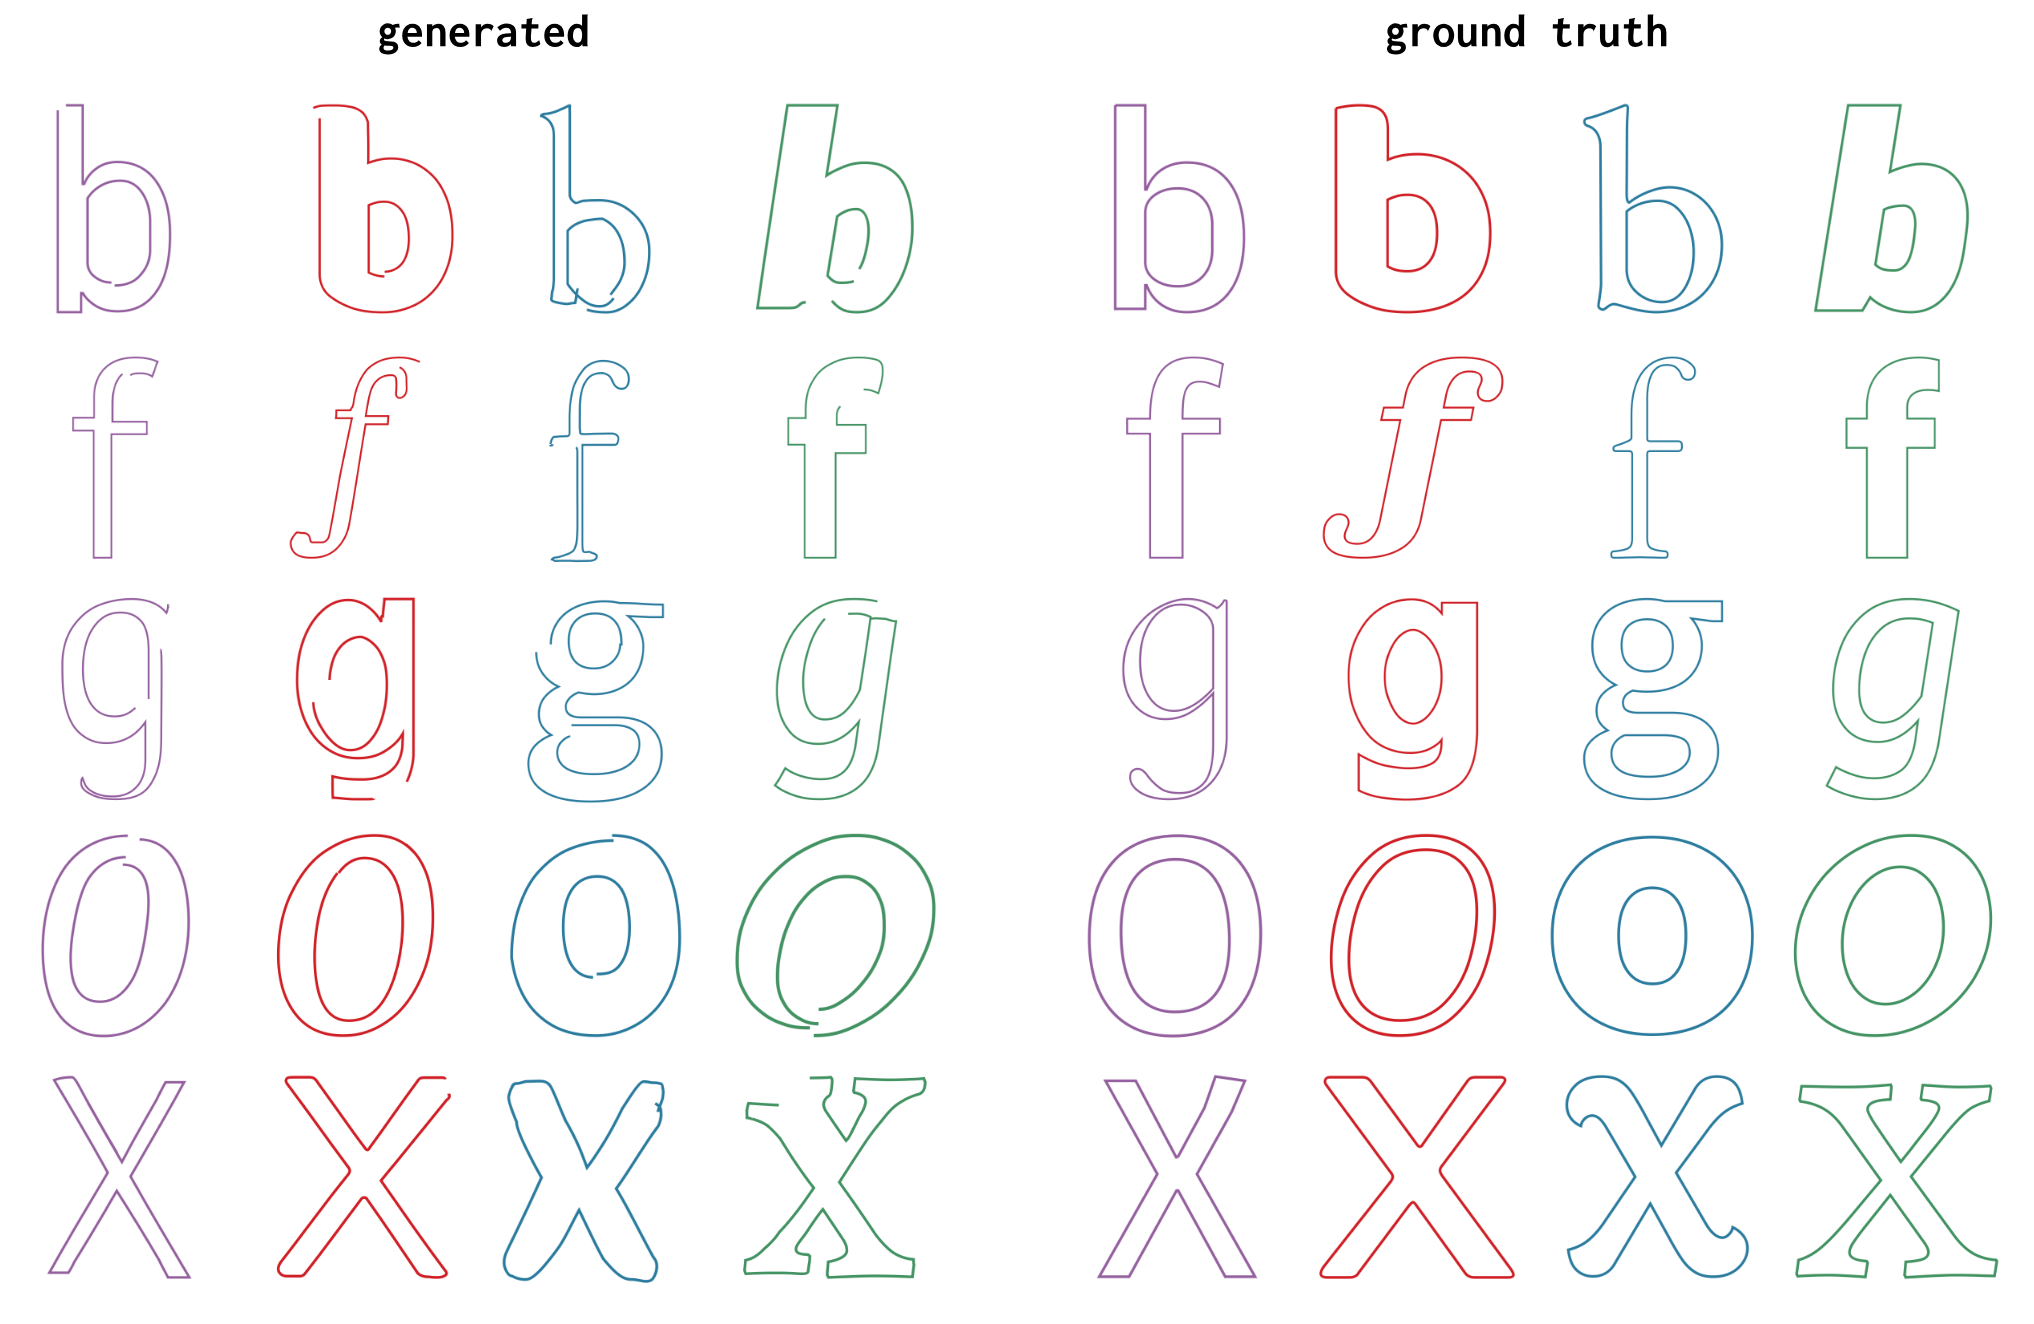
\includegraphics[width=\textwidth]{figures/font_gen}
    \caption[Visual results of training \TODO{blah}]
    \TODO{caption}\label{fig:font_gen}}
\end{figure}

\subsection{Qualitative results}
\begin{figure}[t]
    \centering
	
\includegraphics[width=\textwidth]{figures/temp_grid_b}
    \caption[\TODO{blah}]
    \TODO{caption}\label{fig:temp}}
\end{figure}

\begin{figure}[t]
    \centering
	
\includegraphics[width=\textwidth]{figures/interp}
    \caption[\TODO{blah}]
    \TODO{caption}\label{fig:interp}}
\end{figure}

\TODO{unconditional generation}

\TODO{common failures}
\TODO{vector interpolation}

